\documentclass[acmsmall,review,screen,anonymous]{acmart}

%% TODO during camera-ready
\setcopyright{acmcopyright}
\copyrightyear{2024}
\acmYear{2024}
\acmDOI{XXXXXXX.XXXXXXX}

%% conference information
\acmConference[PLDI'24]{Make sure to enter the correct conference title from
your rights confirmation emai}{June 24--28, 2024}{Copenhagen, Denmark}
\acmPrice{15.00}
\acmISBN{978-1-4503-XXXX-X/18/06}

% load packages
\usepackage{float}
\usepackage{amsmath,amsfonts}
\usepackage{algpseudocode}
\usepackage[ruled, vlined,linesnumbered]{algorithm2e}
\usepackage{graphicx}
\usepackage{textcomp}
\usepackage{xcolor}
\usepackage{soul}
\usepackage{listings}
\usepackage{caption}
\usepackage{subcaption}
\usepackage{multirow}
\usepackage{booktabs}
\usepackage{makecell}
\usepackage{galois}
\usepackage{mathpartir}
\usepackage{bussproofs}
\usepackage{mathtools}
\usepackage{colortbl}
\usepackage{hhline}
\usepackage{stmaryrd}
\usepackage{microtype}
\usepackage{hyperref}
\usepackage{balance}
\usepackage{adjustbox}
\usepackage{tikz}
\usepackage{csquotes}
\usepackage{url}
\usepackage{amstext} % for \text macro
\usepackage{array}   % for \newcolumntype macro

% box
\newcommand{\cfbox}[2]{%
  \colorlet{currentcolor}{.}%
  {\color{#1}%
  \fbox{\color{currentcolor}#2}}%
}
\newcommand{\lcolorbox}[2]{\adjustbox{padding=0ex 1ex 1ex 1ex, bgcolor=#1}{#2}}
\newcommand{\rcolorbox}[2]{\adjustbox{padding=1ex 1ex 0ex 1ex, bgcolor=#1}{#2}}

% table rules
\newcolumntype{?}{!{\vrule width 1pt}}
\newcommand*{\belowrulesepcolor}[1]{%
  \noalign{%
    \kern-\belowrulesep
    \begingroup
      \color{#1}%
      \hrule height\belowrulesep
    \endgroup
  }%
}
\newcommand*{\aboverulesepcolor}[1]{%
  \noalign{%
    \begingroup
      \color{#1}%
      \hrule height\aboverulesep
    \endgroup
    \kern-\aboverulesep
  }%
}

% colors
\definecolor{gainsboro}{rgb}{0.86, 0.86, 0.86}
\definecolor{dkgreen}{rgb}{0, 0.5, 0}
\definecolor{lightred}{rgb}{0.93, 0.57 0.52}
\definecolor{esnt}{rgb}{0.20, 0.20, 0.20}
\definecolor{esparam}{rgb}{0.16, 0.63, 0.59}
\definecolor{esalg}{rgb}{0.12, 0.42, 0.65}
\definecolor{esvar}{rgb}{0.16, 0.63, 0.59}
\definecolor{gray1}{rgb}{0.95, 0.95, 0.95}
\definecolor{gray2}{rgb}{0.85, 0.85, 0.85}
\definecolor{gray3}{rgb}{0.75, 0.75, 0.75}

\newcolumntype{L}{>{$}l<{$}} % math-mode version of "l" column type
\newcommand{\llb}{\llbracket}
\newcommand{\rrb}{\rrbracket}

% basic
\newcommand*{\sphinxDeclareColorOption}[2]{%
   \definecolor{#1}#2%
}%
\sphinxDeclareColorOption{InnerLinkColor}{{rgb}{0.208,0.374,0.486}}
\newcommand{\inblue}[1]{{\color{InnerLinkColor}{#1}}}
%\newcommand{\inblue}[1]{{\color{blue}{#1}}}
\newcommand{\inred}[1]{{\color{red}{#1}}}
\newcommand{\x}[1]{\inred{#1}}
\newcommand{\y}[1]{\textbf{\inred{#1}}}
\newcommand{\todo}{\inred{TODO}}
%\newcommand{\powerset}{\mathcal{P}}
\newcommand{\tif}{\text{if} \; }
\newcommand{\telse}{\text{otherwise}}
\newcommand{\tst}{{\; \text{s.t.} \; }}

% Our tool name
\newcommand{\name}[1]{\textsf{#1}\xspace}
\newcommand{\ssf}[1]{\ensuremath{\mathsf{#1}}\xspace}
\newcommand{\sbf}[1]{\textbf{\small #1}\xspace}
\newcommand{\stt}[1]{\texttt{\small #1}\xspace}
\newcommand{\dsl}{\name{Wasm-DSL}}
\newcommand{\dl}{\name{DL}}
\newcommand{\al}{\name{AL}}
\newcommand{\spectec}{\name{\$SRC}}
\newcommand{\dslname}{SpecTec\xspace}
\newcommand{\ires}{\ssf{IR_{\mathsf{ES}}}}

% codes
\newcommand{\code}[1]{\text{\lstinline[style=JS]!#1!}} 
\newcommand{\scode}[1]{\texttt{\scriptsize #1}} 
\newcommand{\bcode}[1]{\texttt{\small #1}}
\newcommand{\ircode}[1]{\text{\lstinline[style=ires]!#1!}}

\newcommand{\kwsyn}{\bcode{syntax}}
\newcommand{\kwret}{\bcode{return}}

\newcommand{\kwalg}{\bcode{algorithm}}
\newcommand{\kweq}{\coloneqq}
\newcommand{\kwdef}{\bcode{def}}
\newcommand{\kwif}{\bcode{if}}
\newcommand{\kwreturn}{\bcode{return}}
\newcommand{\kweither}{\bcode{either}}
\newcommand{\kwenter}{\bcode{enter}}
\newcommand{\kwassert}{\bcode{assert}}
\newcommand{\kwpush}{\bcode{push}}
\newcommand{\kwpop}{\bcode{pop}}
\newcommand{\kwpopall}{\bcode{popall}}
\newcommand{\kwlet}{\bcode{let}}
\newcommand{\kwtrap}{\bcode{trap}}
\newcommand{\kwnop}{\bcode{nop}}
\newcommand{\kwexecute}{\bcode{execute}}
\newcommand{\kwexecuteseq}{\bcode{executeseq}}
\newcommand{\kwperform}{\bcode{perform}}
\newcommand{\kwexit}{\bcode{exit}}
\newcommand{\kwref}{\bcode{ref}}
\newcommand{\kwreplace}{\bcode{replace}}
\newcommand{\kwiscaseof}{\bcode{iscaseof}}
\newcommand{\kwisdefined}{\bcode{isdefined}}
\newcommand{\kwisvalid}{\bcode{isvalid}}
%\newcommand{\kwwasmc}{\bcode{wasmc}}
%\newcommand{\kw}{\bcode{}}
\newcommand{\kwnot}{\bcode{not}}
\newcommand{\kwequ}{\bcode{=}}
\newcommand{\kwrl}{\bcode{(}}
\newcommand{\kwrr}{\bcode{)}}
\newcommand{\kwcl}{\bcode{\{}}
\newcommand{\kwcr}{\bcode{\}}}
\newcommand{\kwsl}{\bcode{[}}
\newcommand{\kwsr}{\bcode{]}}
\newcommand{\kwass}{\bcode{:=}}
\newcommand{\kwext}{\bcode{:+}}
\newcommand{\kwcat}{\bcode{++}}

\newcommand{\unop}{\ensuremath{\otimes}}
\newcommand{\binop}{\ensuremath{\oplus}}

% Basic
\DeclareMathAlphabet{\mathpzc}{T1}{pzc}{m}{it}
\newcommand{\powerset}[1]{\mathcal{P}(#1)}
\newcommand{\abs}[1]{\widehat{#1}}
\newcommand{\finmap}{{\xrightarrow[]{\text{fin}}}}
\newcommand{\mapstos}{\;\dot{\mapsto}\;}
\newcommand{\Dom}{\name{Dom}}
\DeclarePairedDelimiter{\norm}{\lvert}{\rvert} 

% JavaScript
\newcommand{\js}{\name{js}}

% Getters
\newcommand{\getfunc}{\name{func}}
\newcommand{\getinst}{\name{inst}}
\newcommand{\getnext}{\name{next}}
\newcommand{\getcaller}{\name{caller}}
\newcommand{\getlab}{\name{label}}

% Values
\newcommand{\valset}{\mathbb{V}}
\newcommand{\val}{v}
\newcommand{\pvalset}{\valset^\name{p}}
\newcommand{\pval}{\val^\name{p}}
\newcommand{\boolset}{\valset_\name{bool}}
\newcommand{\bool}{b}
\newcommand{\true}{\code{\#t}}
\newcommand{\false}{\code{\#f}}
\newcommand{\intset}{\valset_\name{int}}
\newcommand{\strset}{\valset_\name{str}}

% JavaScript ASTs
\newcommand{\treeset}{\mathbb{T}}
\newcommand{\tree}{t}
\newcommand{\trees}{\overline{t}}
\newcommand{\nodeset}{\Phi}
\newcommand{\node}{\phi}
\newcommand{\subtree}{\lhd}
\newcommand{\getsubs}{\name{subs}}
\newcommand{\treetop}{\code{\#}}
\newcommand{\ty}{\tau}
\newcommand{\eval}{\code{eval}}

% DL Syntax
\newcommand{\defnset}{\mathfrak{D}}
\newcommand{\defn}{d}
\newcommand{\infrset}{\mathcal{R}}
\newcommand{\infr}{r}
\newcommand{\funcset}{\mathcal{F}}
\newcommand{\func}{f}

% AL Syntax
\newcommand{\progset}{\mathfrak{P}}
\newcommand{\prog}{p}
\newcommand{\algset}{\mathcal{A}}
\newcommand{\alg}{a}
\newcommand{\instset}{\mathcal{I}}
\newcommand{\inst}{i}
\newcommand{\exprset}{\mathcal{E}}
\newcommand{\expr}{e}
\newcommand{\condset}{\mathcal{C}}
\newcommand{\cond}{c}
\newcommand{\numset}{\mathcal{N}}
\newcommand{\num}{n}
\newcommand{\qualset}{\mathcal{Q}}
\newcommand{\qual}{q}
\newcommand{\wasmcset}{\mathcal{W}}
\newcommand{\wasmc}{w}
\newcommand{\cnstrset}{\mathcal{K}}
\newcommand{\cnstr}{k}

% Variables
\newcommand{\varset}{\mathcal{X}}
\newcommand{\varx}{x}
\newcommand{\varf}{f}
\newcommand{\vart}{t}
\newcommand{\varp}{p}

% Field Mappings
\newcommand{\fmapset}{\mathbb{M}}
\newcommand{\fmap}{m}
\newcommand{\jsfmapset}{\fmapset_\js}
\newcommand{\jsfmap}{\fmap_\js}

% Transition Relations
\newcommand{\trans}[1]{\leadsto_{#1}}

\newcommand{\hide}[1]{}
\newcommand{\unify}{\ensuremath{\mathcal{U}}\xspace}
\newcommand{\dltoil}{\ensuremath{\mathcal{T}}\xspace}


\begin{document}

\title[Bringing the WebAssembly Standardization up to Speed]
{Bringing the WebAssembly Standardization up to Speed with \dslname}

%% authors
%% abstract

%% TODO http://dl.acm.org/ccs.cfm during camera ready
% \begin{CCSXML}
% <ccs2012>
%  <concept>
%   <concept_id>10010520.10010553.10010562</concept_id>
%   <concept_desc>Computer systems organization~Embedded systems</concept_desc>
%   <concept_significance>500</concept_significance>
%  </concept>
%  <concept>
%   <concept_id>10010520.10010575.10010755</concept_id>
%   <concept_desc>Computer systems organization~Redundancy</concept_desc>
%   <concept_significance>300</concept_significance>
%  </concept>
%  <concept>
%   <concept_id>10010520.10010553.10010554</concept_id>
%   <concept_desc>Computer systems organization~Robotics</concept_desc>
%   <concept_significance>100</concept_significance>
%  </concept>
%  <concept>
%   <concept_id>10003033.10003083.10003095</concept_id>
%   <concept_desc>Networks~Network reliability</concept_desc>
%   <concept_significance>100</concept_significance>
%  </concept>
% </ccs2012>
% \end{CCSXML}
%
% \ccsdesc[500]{Computer systems organization~Embedded systems}
% \ccsdesc[300]{Computer systems organization~Redundancy}
% \ccsdesc{Computer systems organization~Robotics}
% \ccsdesc[100]{Networks~Network reliability}
\keywords{
  WebAssembly,
  language specification,
  executable prose,
  DSL
}

\maketitle

%% body of the paper
\section{Introduction}\label{sec:intro}
\begin{figure}[t]
  \centering
  \begin{subfigure}{\textwidth}
    \centering
    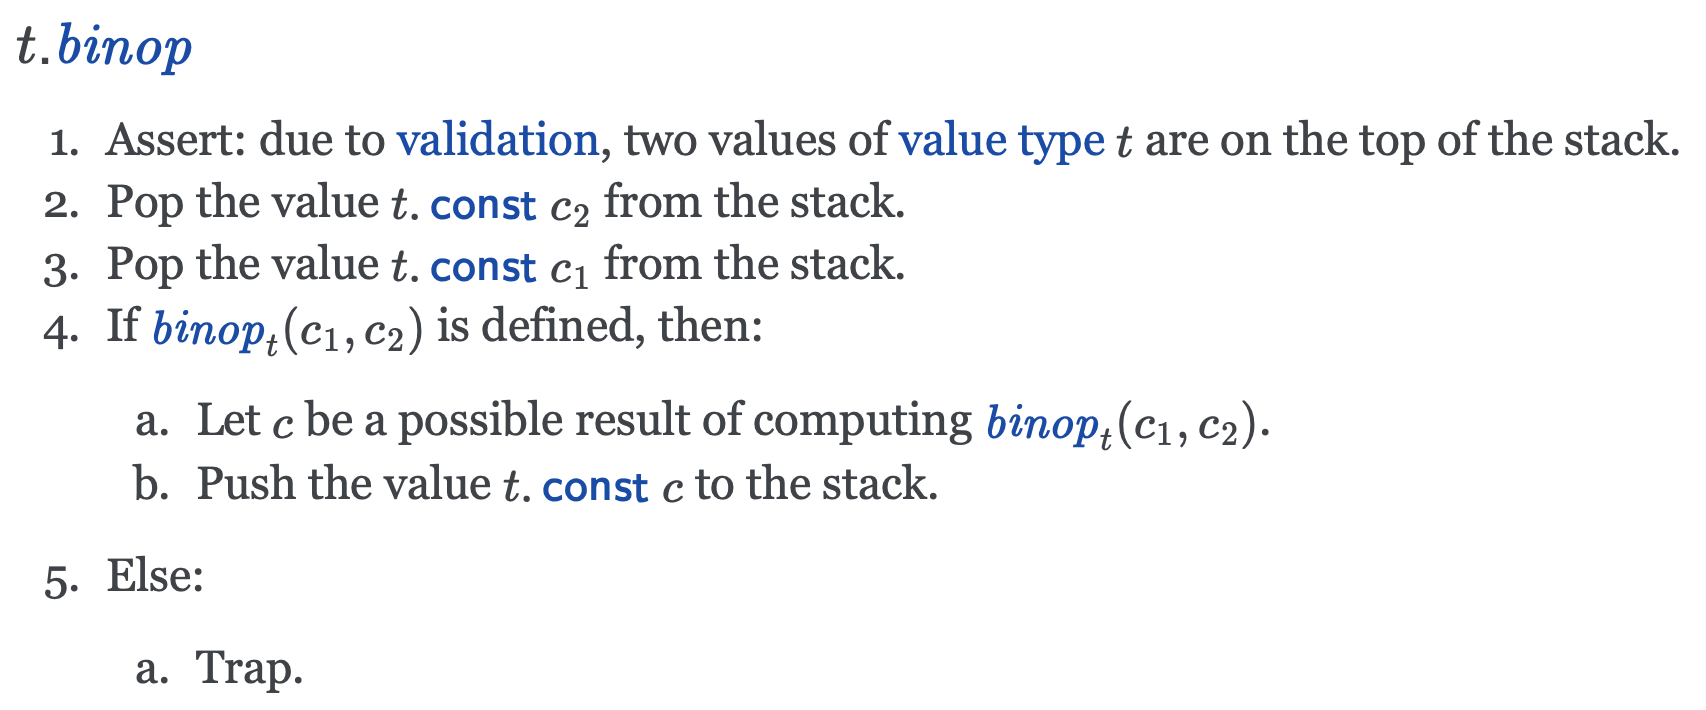
\includegraphics[width=.7\textwidth]{../img/spec-prose.png}
\vspace*{-1em}
    \subcaption{Prose notation}
\vspace*{.5em}
  \end{subfigure}
  \begin{subfigure}{\textwidth}
    \centering
    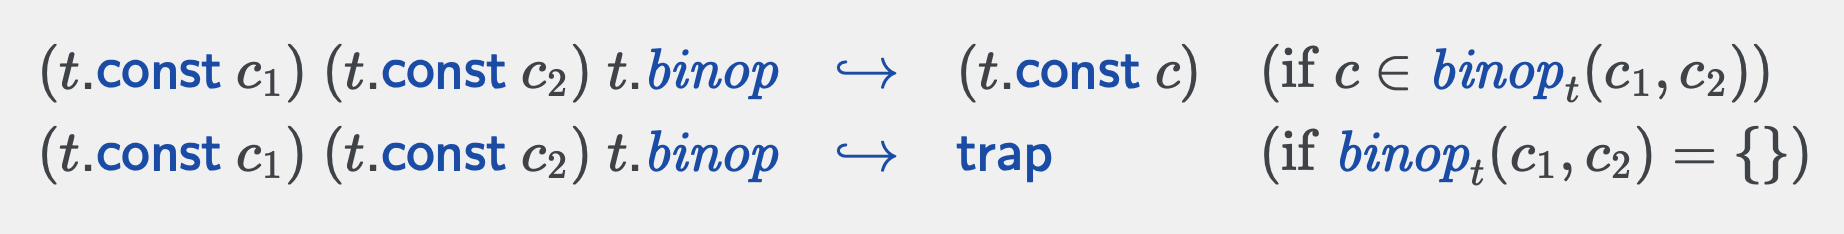
\includegraphics[width=.7\textwidth]{../img/spec-formal.png}
    \subcaption{Formal notation}
  \end{subfigure}
\caption{Semantics of \ensuremath{t.\mathit{\inblue{binop}}} in the specification}
\label{fig:spec}
\end{figure}

A programming language is defined by its syntax and semantics.
Syntax and semantics are the basis for all subsequent development and
analysis of the language, so it is important to define them clearly and rigorously. 
Many programming languages, such as Java~\cite{javaspec} and Python~\cite{pythonspec},
therefore have language specifications that define their syntax and semantics.
For languages that are prone to implementation inconsistency issues,
such as C~\cite{cstandard} and JavaScript~\cite{ecmascript},
international committees define them according to their own standardization processes.
Some languages, like Standard ML~\cite{sml}, even have formal descriptions
that define them in mathematical notation.

WebAssembly (Wasm) is a low-level bytecode language and virtual machine~\cite{wasmspec}.
It was initially designed as an efficient compilation target and execution model on Web platforms
and has been adopted across a wide range of ecosystems,
including cloud and edge computing~\cite{lucet, cloudflare}, 
mobile and embedded systems~\cite{wasm-embedded}, IoT~\cite{wasm-iot}, and
blockchains~\cite{wasm-blockchain}.
Because different browsers implement Wasm within vendor-specific architectures
using multi-tier interpretation or just-in-time compilation,
Wasm faces the risk of implementation discrepancies.
The diversity of the various ecosystems exacerbates the situation.

To mitigate these risks, Wasm has been standardized by
the W3C Wasm Community Group~\cite{wasm-w3c}.
It requires four key artifacts for a feature to be standardized:
1) a \textit{formal specification} for the feature in declarative-style rewrite rules, written in LaTeX;
2) a \textit{prose pseudocode} presenting an algorithmic-style semantics, written in reStructuredText markup;
3) an extended \textit{reference interpreter} with the implementation of the feature, written in OCaml; and
4) a \textit{unit test suite} for the feature, written in the Wasm text format.
All of these artifacts must define the same behavior of a Wasm program.
Note that the specification provides \textit{both} declarative and algorithmic styles of semantic definitions.
For example, Fig.~\ref{fig:spec} shows the execution semantics of the binary operation instruction
$t.\mathit{\inblue{binop}}$ in the official Wasm specification.
Fig.~\ref{fig:spec}(a) presents the semantics in a prose notation broken down into five steps,
while Fig.~\ref{fig:spec}(b) specifies it in a formal notation using rewrite rules.

The two styles of semantic definitions cater to the dual needs of
language ``designers'' and ``implementers.''  Declarative rewrite
rules serve the needs of designers by focusing on clarity and
correctness of language semantics. They allow theorem provers like
Coq, Isabelle, Lean, and Agda to mechanize language semantics
and prove various properties, including type safety.
Algorithmic prose pseudocode, on the other hand, helps implementers
understand language behavior. A step-by-step description of the
language semantics can be a good guide to how to implement it.

Despite the onerous standardization process, the Wasm specification has been
written and maintained \textit{manually}, which creates challenges for specification writers.
Writing the prose is extremely laborious~\cite{Andreasicfp23}, and code reviews of
feature proposals written in LaTeX and reStructuredText are not user-friendly.
Manual processes are vulnerable to human error, potentially leading
to inconsistencies or inaccuracies in the specification.
As Wasm grows with new language features such as Garbage Collected Types, Threads,
and Exception Handling that will be supported by Wasm 3.0,
manually crafting all of the artifacts is not scalable.

These challenges call for the need to automate the process or \textit{mechanize} the language semantics.
For declarative-style rewrite rules, the literature shows general-purpose language frameworks such as
Ott~\cite{ott}, PLTRedex~\cite{pltredex}, Skeleton~\cite{skeleton}, Spoofax~\cite{spoofax},
and the K framework~\cite{k}. Among them, the K framework can generate various tools,
including interpreters, model checkers, and verifiers, from a language specification written in its language K.
It has specified the core semantics of real-world programming languages
such as C~\cite{kc}, Java~\cite{kjava}, Python~\cite{kpython}, and JavaScript~\cite{kjs}.
For algorithmic-style semantics, the ESMeta framework~\cite{esmeta}
can extract a mechanized specification from
an ECMAScript/JavaScript specification~\cite{ecmascript} and automatically
generate diverse tools~\cite{jiset,jest,jstar,jsaver}.
%
%  ESMeta parses the structured English prose algorithms of ECMAScript
% Specification document, and translates them into an internal representation, $IR_{ES}$.
%   $IR_{ES}$ has its own semantics, and thus can be executed with an interpreter implementation.
%   Executing the JavaScript semantics written in $IR_{ES}$ allows an indirect execution of JavaScript programs.
%   Utilizing the executable semantics, ESMeta derives a type checker for the specification, test
% suite synthesizers, and a static analyzer of JavaScript.
%
% Now, each ECMA-262 PR will execute the ESMeta type checker, and any new or changed tests in a Test262 PR will be executed using the ESMeta interpreter.
%
ESMeta has been officially integrated into the continuous integration (CI) systems of
the ECMAScript specification~\cite{ciecma262} and the Test262 conformance test suite~\cite{citest262}
since November 2022.
Because the existing language frameworks can mechanize only one style of semantics,
they are not applicable to Wasm, which should support both declarative and algorithmic styles of semantics.

\begin{figure}[t]
\footnotesize
\begin{verbatim}
                rule Step_pure/binop-val:
                    (CONST nt c_1) (CONST nt c_2) (BINOP nt binop) ~> (CONST nt c)
                    -- if $binop(binop, nt, c_1, c_2) = c

                rule Step_pure/binop-trap:
                    (CONST nt c_1) (CONST nt c_2) (BINOP nt binop) ~> TRAP
                    -- if $binop(binop, nt, c_1, c_2) = epsilon
\end{verbatim}
\caption{The binary operator semantics in \spectec's DSL}
\label{fig:dsl}
\end{figure}

In this paper, we propose \spectec, a framework for mechanizing Wasm semantics in both styles.
\spectec presents a \emph{Domain-Specific Language (DSL)} that
defines the Wasm syntax, type system, and execution semantics in a declarative style,
which serves as a single source of truth.
Figure~\ref{fig:dsl} illustrates the semantics of $t.\mathit{\inblue{binop}}$ in the DSL,
which looks similar to the one in the official specification in Figure~\ref{fig:spec}(b).
Once the Wasm formal semantics is written in the DSL,
a number of tools can be automatically generated as backends:
1) declarative backends, including LaTeX-based formal specifications and
mechanized definitions in various theorem provers, and
2) algorithmic backends, such as prose specifications in reStructuredText and Wasm interpreters.
By conducting meta-level error checking and automatically generating the required specification artifacts,
\spectec can alleviate the burden on language designers and implementers.

\spectec's DSL is designed to provide a close and easy representation and reasoning of
the Wasm semantics in declarative backends.
It can directly produce LaTeX-based formal specifications from the definitions in the DSL,
and all definitions and variables in the DSL are ``type-checked'' to detect ill-formed ones.
It can also generate mechanized definitions for theorem provers.
This saves language designers the trouble of manually specifying
language semantics in different theorem provers every time the specification is updated.

On the contrary, algorithmic backends are not directly produced from the definitions in the DSL,
but from the definitions in the \emph{Algorithmic Language (AL)}.
The AL is designed to provide a close and easy representation and manipulation of
the Wasm semantics in the official prose specification,
so the English prose in reStructuredText markup can be generated directly from the definitions in the AL.
\spectec can also support the interpretation of Wasm programs,
following the approach of the ESMeta framework.

To bridge the gap between the two styles of semantics,
we present a mechanism for automatically deriving algorithmic ALs from declarative DSLs.
Several challenges arise in transforming declarative-style rewrite rules
into algorithmic-style prose pseudocode.
For example, a single Wasm instruction may have multiple rewrite rules,
each expressing certain premises,
but each instruction should have only one prose pseudocode. 
In addition, the equals operator `$=$' in mathematical rules
can be ambiguous, as it can mean assignment or equality checking.
We show that the transformation is an NP-hard problem
and propose a practical solution.

\spectec is available as an open-source project~\cite{spectec}
and covers everything in Wasm 2.0 except SIMD instructions.
The automatically generated Wasm semantics in the AL passes
100\% of the official test suite (except for SIMD) using an AL interpreter.
To further specify the semantics for Wasm 3.0, we only needed
to make minor adjustments in \spectec. During this process, we
reported a few errors in the Garbage Collected Types proposal and
received confirmation from the proposal champions.

This paper presents the following contributions:
\begin{itemize}
\item \textbf{\spectec is the first language semantics framework that
embraces both declarative and algorithmic styles of semantics.}
Unlike existing language frameworks that can mechanize only one style of semantics,
\spectec can support both styles of semantics.

\item \textbf{\spectec can automatically generate multiple backends from 
a single source of truth.}
It is designed to be easy to write, read, and reivew, enabling
meta-level error detection in the Wasm specification.

\item \textbf{\spectec is a forward-compatible toolchain that can
adapt to the evolving Wasm semantics.}
To evaluate \spectec's forward compatibility, we applied it to five
proposals in Wasm 3.0 and found that only minor adjustments were necessary. 
\end{itemize}

\section{Algorithmic Backends}\label{sec:al}
This section presents a mechanism for automatically generating
algorithmic backends from the formal semantics.
We define \emph{\dl}, a declarative language that defines the formal
semantics of Wasm (Sec.~\ref{sec:dl}),
\emph{\al}, an algorithmic language that defines the Wasm semantics
in a pseudocode style (Sec.~\ref{sec:aldef}),
and a \dl to \al transformation (Sec.~\ref{sec:dl2al}).
We then show how to generate a prose specification from the semantics
described in \al (Sec.~\ref{sec:prose}) and
support its interpretation (Sec.~\ref{sec:interp}).

\subsection{\dl: Declarative Language}\label{sec:dl}
The DSL describes the formal semantics of Wasm, and
we abstract it into a \dl that only shows the features relevant to translation to an algorithmic representation.
Fig.~\ref{fig:dl-syntax} presents the syntax of \dl.

\begin{figure}[t]
\[
\small
\begin{array}{l@{~}c@{~}r@{~}l}
\text{Semantics} & \delta^*\\
\text{Definition} & \delta &::=& \rho\ \mid\ \lambda\\
\text{Reduction rule} & \rho &::=& \gamma \leadsto \gamma\ \mbox{---}\ \pi^*\\
\text{Configuration} & \gamma &::=&(\eta_\bot,\ \eta)\\
\text{Premise} & \pi &::=& \beta\ \mid\ \mathsf{\small otherwise}\\
\text{Helper function} &
\lambda &::=& \varx \kwrl \eta^* \kwrr\ \kwequ\ \eta\ \mbox{---}\ \pi^*\\
\text{Expression} & \eta &::=& \upsilon\ \mid\ \kappa\ \eta^*\ \mid\ \eta + \eta\
\mid \eta^*\ \mid \eta \leftarrow \eta \ \mid (\eta,\ \eta)\
\mid \cdots \\
\text{Condition} & \beta  &::=& \eta\ = \eta\ \mid \cdots\\
\text{Value} & \upsilon &::=& \ssf{I32}\ \mid\ \ssf{I64}\ \mid\ 
\ssf{F32}\ \mid\ \ssf{F64}\ \mid\ 
\ssf{0}\ \mid\ \ssf{1}\ \mid\ x\ \mid\ \epsilon\ \mid \cdots \\
\text{Constructor} & \kappa &::=& \ssf{REF.IS\_NULL}\ \mid\ \ssf{REF.NULL}\
\mid\ \ssf{REF} \mid\ \ssf{NULL}\ \mid\ \ssf{CONST}\ \mid\ \ssf{LABEL\_}\
\mid\ \ssf{BR}\
\mid \cdots
\end{array}
\]
\caption{Syntax of \dl for Wasm}\label{fig:dl-syntax}
\end{figure}

The Wasm semantics is defined by a sequence of definitions $\delta^*$.
A definition is either a reduction rule $\rho$ or an auxiliary helper function $\lambda$.
A reduction rule $\gamma_1 \leadsto \gamma_2\ \mbox{---}\ \pi^*$ denotes that
when the current configuration of a program matches $\gamma_1$ and
all $\pi^*$ are evaluated to true, then the program configuration becomes $\gamma_2$.
A configuration $(\eta_\bot,\ \eta)$ denotes an optional Wasm program state $\eta_\bot$,
which is a pair of the current store and the current frame,
and a Wasm instruction $\eta$ that represents the current stack.
Because the details of the Wasm program states and instructions are
not relevant to this paper,
we abstract them as $\eta$. We show only some cases used for concrete
examples in this paper.
A premise $\pi$ is a condition $\beta$ or a special keyword
\ensuremath{\mathsf{\small otherwise}},
which denotes the negation of all the previous premises.
We also abstract the details of the Wasm conditions as $\beta$.
A helper function $\varx \kwrl \eta^* \kwrr\ \kwequ\ \eta\ \mbox{---}\ \pi^*$ denotes that
when a function named $\varx$ is called, its arguments are bound to parameters $\eta^*$
and a body expression $\eta$ is evaluated if all $\pi^*$ are evaluated to true.

For example, the semantics of \inblue{\ensuremath{\mathsf{ref.is\_null}}}
in Fig.~\ref{fig:dsl} corresponds to the following in \dl:
\[
\begin{array}{l@{}l@{~}c@{~}l}
[&(\bot, [\upsilon, \ssf{REF.IS\_NULL}]) &\leadsto& (\bot, [\ssf{CONST\ I32\ 1}])\
\mbox{---}\ [\upsilon = \ssf{REF.NULL}\ t],\\
&(\bot, [\upsilon, \ssf{REF.IS\_NULL}])&\leadsto&(\bot, [\ssf{CONST\ I32\ 0}])\
\mbox{---}\ [\ssf{\small otherwise}] ]
\end{array}
\]
where a sequence is represented as comma separated elements
enclosed by $[$ and $]$ for readability.

\subsection{\al: Algorithmic Language}\label{sec:aldef}
Before generating algorithmic backends, definitions in \dl are translated into definitions in \al,
an algorithmic language that defines the Wasm language semantics in a pseudocode style.

\begin{figure}[t]
\[
\small
\begin{array}{l@{~}r@{~}c@{~}c@{~}r@{~}lll}
\text{Program} & \progset &\ni& \prog &::=& \alg^*\\
\text{Algorithm} & \algset &\ni& \alg &::=&
\kwalg \; \varx \kwrl \expr^* \kwrr \; \kwcl \inst^* \kwcr \\
\text{Instruction} & \instset &\ni& \inst &::=&
    \kwif \; \cond \; \inst^* \; \inst^* & \mbox{If $\cond$, then: $\inst_1^*$ Else: $\inst_2^*$}\\
&&&& \mid&
    \kweither \; \inst^* \; \inst^* & \mbox{Either: $\inst_1^*$ Or: $\inst_2^*$}\\
&&&& \mid&
    \kwenter \; \expr \; \expr \; \inst^* & \mbox{Enter $\expr_1$ with label $\expr_2$\ :\ $\inst^*$}\\
&&&& \mid&
    \kwassert \; \cond  & \mbox{Assert: Due to validation, $\cond$.}\\
&&&& \mid&
    \kwpush \; \expr  & \mbox{Push $\expr$ to the stack.}\\
&&&& \mid&
    \kwpop \; \expr  & \mbox{Pop $\expr$ from the stack.}\\
&&&& \mid&
    \kwpopall \; \expr  & \mbox{Pop all values $\expr$ from the stack.}\\
&&&& \mid&
    \kwlet \; \expr \; \expr & \mbox{Let $\expr_1$ be $\expr_2$.}\\
&&&& \mid&
    \kwtrap & \mbox{Trap.}\\
&&&& \mid&
    \kwnop & \mbox{Do nothing.}\\
&&&& \mid&
    \kwreturn \; \expr^? & \mbox{Return $\expr^?$.}\\
&&&& \mid&
    \kwexecute \; \expr & \mbox{Execute $\expr$.}\\
&&&& \mid&
    \kwexecuteseq \; \expr & \mbox{Execute the sequence $\expr$.}\\
&&&& \mid&
    \kwperform \; \varx \; \expr^* & \mbox{Perform $\varx(\expr^*)$.}\\
&&&& \mid&
    \kwexit & \mbox{Exit current context.}\\
&&&& \mid&
    \kwreplace \; \expr \; \qual \; \expr & \mbox{Replace $\expr_1[\qual]$ with $\expr_2$.}
\\

\text{Expression} & \exprset &\ni& \expr &::=&
    \varx & \varx\\
&&&& \mid&
    \num & \num\\
&&&& \mid&
    \bcode{-} \; \expr & \bcode{-} \; \expr\\
&&&& \mid&
    \expr \; \binop \; \expr & \expr \; \binop \; \expr\\
&&&& \mid&
    \expr \kwsl \qual \kwsr & \expr \kwsl \qual \kwsr\\
&&&& \mid&
    \expr \kwsl \qual \kwsr \; \kwass \; \expr & \mbox{$\expr_1$ with $\qual$ replaced by $\expr_2$}\\
&&&& \mid&
    \expr \kwsl \qual \kwsr \; \kwext \; \expr & \mbox{$\expr_1$ with $\qual$ prepended/appended by $\expr_2$}\\
&&&& \mid&
    \kwcl (\varx \mapsto \expr)^* \kwcr & \{\ (\varx~\expr)^*\ \}\\
&&&& \mid&
    \expr \; \kwcat \; \expr & \expr_1~\expr_2\\
&&&& \mid&
    | \expr | & |\expr|\\
&&&&&& \mbox{the length of $\expr$}\\
&&&&\mid&
    \cnstr \kwrl \expr^* \kwrr & \cnstr(\expr^*)\\
&&&& \mid&
    \varx \kwrl \expr^* \kwrr & \varx~\expr^*\\
&&&& \mid&
    \wasmc \\

\text{Condition} & \condset &\ni& \cond &::=&
\multicolumn{2}{l}{
    \kwnot \; \cond \mid
    \cond \; \binop \; \cond \mid
    \expr \; \binop \; \expr \mid
    \kwiscaseof \; \expr \; \varx \mid
    \kwisdefined \; \expr \mid
    \kwisvalid \; \expr \mid
    \wasmc
}
\\

\text{Path} & \qualset &\ni& \qual &::=&
\multicolumn{2}{l}{
    \expr \mid
    \expr \bcode{:} \expr \mid
    \bcode{.} x
}
\\
%\text{Wasm} & \wasmcset &\ni& \wasmc \\
  % Wasm-specific condition
  % (* Conditions used in assertions *)
  % | TopLabelC                        (* "a label is now on the top of the stack" *)
  % | TopFrameC                       (* "a frame is now on the top of the stack" *)
  % | TopValueC of expr option (* "a value (of type expr)? is now on the top of the stack" *)
  % | TopValuesC of expr           (* "at least expr number of values on the top of the stack" *)
  \end{array}
\]
\vspace*{-1em}
\caption{Syntax of \al and its prose notation}\label{fig:al-syntax}
\end{figure}

Fig.~\ref{fig:al-syntax} presents the core syntax of \al.
The metavariables $\varx$ ranges over variables,
$\num$ ranges over numbers, and
$\cnstr$ ranges over constructors.
An \al program $\prog$ is a sequence of algorithms $\alg^*$,
which denotes the Wasm semantics.
An algorithm $\alg$ consists of a name $\varx$, parameters $\expr^*$,
and body instructions $\inst^*$, which denotes the semantics of a
language feature or a helper function used to describe the language semantics.
An instruction $\inst$ denotes a prose statement in the Wasm specification.
The figure also shows prose rendering of instructions and expressions.
The Wasm specification often uses specific phrases like ``the current frame'' and 
``a label is now on the top of the stack.''
We abstract such Wasm-specific expressions and conditions as $\wasmc$ for brevity.
Note that an \al expression may have a different prose rendering
depending on where it appears. For example, $|e|$ is rendered as 
``$|\expr|$'' or ``the length of $\expr$'' depending on whether it appears in
a mathematical context or not.
To support intuitive prose notation, some \al conditions are specially rendered.
For example, while ``$\kwnot$'' is rendered as ``not'' and ``$\kwisvalid\;\expr$''
is rendered as ``$\expr$ is valid,''
``$\kwnot \; (\kwisvalid \; \expr)$'' is rendered as ``$\expr$ is not valid''
rather than ``not $\expr$ is valid.''

For example, the semantics of \inblue{\ensuremath{\mathsf{ref.is\_null}}}
in Fig.~\ref{fig:dsl} corresponds to the following in \al:
\[
\small
\!\!
\begin{array}{r@{~}l}
\kwalg \; \mathit{REF.IS\_NULL} \kwrl \kwrr \; \kwcl &
  \kwassert \; \wasmc \\
& \kwpop \; \mathit{val}\\
& \kwif \; (\kwiscaseof \; \mathit{val} \; \mathit{REF.NULL})\;
\; (\kwpush \; \ssf{CONST}(\ssf{I32}(1))) \; (\kwpush \; \ssf{CONST}(\ssf{I32}(0)))\\
\kwcr
\end{array}
\]

\subsection{\dl to \al Transformation}\label{sec:dl2al}
Now, we describe how to transform a Wasm semantics $\delta^*$ in \dl into an \al program $\prog$.
First, the definitions in $\delta^*$ are grouped to represent algorithms; among $\delta^*$,
the reduction rules $\gamma^*$ are grouped according to their target Wasm instructions, and
the helper functions $\lambda^*$ are grouped according to their names.
Each group is transformed into a single algorithm in two phases:
1) preprocess the group's definitions to satisfy some \textit{preconditions}, and
2) generate an \al algorithm from the preprocessed \dl definitions.

\subsubsection{\dl to \dl Preprocessing}
Preprocessing consists of two steps: for each group of reduction rules (or helper functions),
1) preprocess the left-hand sides (or parameters) of the reduction rules (or helper functions)
in the group to make them the same, and
2) preprocess the premises of the definitions in the group
so that every variable is bound exactly once before its uses.

\medskip
The first preprocessing step is to make the left-hand sides (or parameters) of
the reduction rules (or helper functions) in each group identical.
Most Wasm  definitions satisfy this precondition, but some do not, such as the following
DSL reduction rules for the \inblue{\ensuremath{\mathsf{br}}} instruction:

{
\begin{verbatim}
     rule Step_pure/br-zero:
        (LABEL_ n `{instr'*} val'* val^n (BR 0) instr*)  ~>  val^n instr'*

     rule Step_pure/br-succ:
        (LABEL_ n `{instr'*} val* (BR $(l+1)) instr*)  ~>  val* (BR l)
\end{verbatim}
}

\noindent
which corresponds to the following in \dl:
\[
\begin{array}{l@{~}l@{~}c@{~}l}
\rho_1 = &(\bot, (\ssf{LABEL\_} \; n) \; \eta'^*\; v'^*\; v^n\; (\ssf{BR\; 0})\; \eta^*) &\leadsto&
 (\bot,\; v^n\; \eta^*)\ \mbox{---}\ []\\
\rho_2 = &(\bot, (\ssf{LABEL\_} \; n) \; \eta'^*\; v^*\; (\ssf{BR\; (}l\ssf{+1)})\; \eta^*) &\leadsto&
 (\bot,\; v^*\; (\ssf{BR}\; l))\ \mbox{---}\ []
\end{array}
\]

For each group of reduction rules $\rho^* =
(\eta_1, \eta' _1) \leadsto \gamma_1\ \mbox{---}\ \pi_1^*\
\cdots\
(\eta_n, \eta' _n) \leadsto \gamma_n\ \mbox{---}\ \pi_n^*$,
the unification algorithm \unify takes a list of expressions to unify,
$\eta_1\,\eta'_1\ \cdots\ \eta_n\,\eta'_n$, and returns a pair of
a unified expression $\eta$ and a list of premises $\pi^n$.
Similarly, for each group of helper functions $\lambda^*=
\varx_1 \kwrl \eta_1^* \kwrr\ \kwequ\ \eta_1\ \mbox{---}\ \pi_1^*\
\cdots\
\varx_n \kwrl \eta_n^* \kwrr\ \kwequ\ \eta_n\ \mbox{---}\ \pi_n^*$,
\unify takes a list of expressions to unify,
$\eta_1^*\ \cdots\ \eta_n^*$, and returns a pair of
a unified expression $\eta$ and a list of premises $\pi^n$.
For the \inblue{\ensuremath{\mathsf{br}}} instruction, for example,
\unify takes two expressions
``{$(\ssf{LABEL\_} \; n) \; \eta'^*\; v'^*\; v^n\; (\ssf{BR\; 0})\; \eta^*$}'' and
``{$(\ssf{LABEL\_} \; n) \; \eta'^*\; v^*\; (\ssf{BR\; (}l\ssf{+1)})\; \eta^*$}.''

For a list of expressions to unify $\eta_1\ \cdots\ \eta_n$,
\unify first 1) generates a unified expression $\eta$ possibly containing some fresh variables
and then 2) generates premises $\pi_i^*\ (1\le i \le n)$ using the fresh variables to make
each $\eta_i\ (1\le i \le n)$ be the same as $\eta$ with $\pi_i^*\ (1\le i \le n)$.
More specifically, the unified expression $\eta$ is the most common expression of
the expressions to unify $\eta_1\ \cdots\ \eta_n$,
replacing the different components with fresh variables.
For example, the unified expression for the reduction rules for \inblue{\ensuremath{\mathsf{br}}} is
``{$(\ssf{LABEL\_} \; n) \; \eta'^*\; t\; (\ssf{BR}\; t')\; \eta^*$}.''
After generating the unified expression, \unify generates premises $\pi_i^*\ (1\le i \le n)$
for each $\eta_i\ (1\le i \le n)$ so that $\eta_i$ is an instance of the unified expression satisfying $\pi_i^*$.
For $\eta_i\ (1\le i \le n)$, \unify infers the conditions $\pi_i^*$ for the free variables
in the unified expression $\eta$ to make $\eta$ the same as $\eta_i$.
For example, to make the unified expression for \inblue{\ensuremath{\mathsf{br}}}
same as the left-hand sides of $\rho_1$ and $\rho_2$, \unify infers the conditions
$[t = v'^*\; v^n,\ t' = 0]$ and $[t = v^*,\ t' = l\ssf{+1}]$, respectively.
Finally, the unification result of the rules for the \inblue{\ensuremath{\mathsf{br}}} instruction is as follows:
\[
\begin{array}{l@{~}l@{~}c@{~}l}
\rho_1 = &(\bot, (\ssf{LABEL\_} \; n) \; \eta'^*\; t\; (\ssf{BR}\; t')\; \eta^*) &\leadsto&
 (\bot, v^n\; \eta^*)\ \mbox{---}\ [t = v'^*\; v^n,\ t' = 0]\\
\rho_2 = &(\bot, (\ssf{LABEL\_} \; n) \; \eta'^*\; t\; (\ssf{BR}\; t')\; \eta^*) &\leadsto&
 (\bot, v^*\; (\ssf{BR}\; l))\ \mbox{---}\ [t = v^*,\ t' = l\ssf{+1}]
\end{array}
\]
The fresh variables $t$ and $t'$ are introduced for both rules $\rho_1$ and $\rho_2$
to make their left-hand sides the same. The definitions of $t$ and $t'$ are available as premises:
$[t = v'^*\; v^n,\ t' = 0]$ for $\rho_1$ and
$[t = v^*,\ t' = l\ssf{+1}]$ for $\rho_2$.


\medskip
The second preprocessing step is to change the premises of each group's definitions
so that each variable is bound exactly once before it is used.
While the order of the premises is not important in declarative reduction rules,
it is crucial in algorithmic backends.
In addition, an equality expression $\eta = \eta'$ in a premise $\pi$ can be ambiguous,
because it can refer to an equality check condition or a variable binding.
This second preprocessing step replaces every equality expression denoting a variable binding with $\eta \leftarrow \eta'$.
Thus, this step identifies each variable's binding occurrence,
keeps track of the variables that each premise binds,
and reorders premises so that preceding premises bind all free variables in each premise.

For example, consider the rules for the \inblue{\ensuremath{\mathsf{br}}} instruction again:
\[
\begin{array}{l@{~}l@{~}c@{~}l}
\rho_1 = &(\bot, (\ssf{LABEL\_} \; n) \; \eta'^*\; t\; (\ssf{BR}\; t')\; \eta^*) &\leadsto&
 (\bot, v^n\; \eta^*)\ \mbox{---}\ [t = v'^*\; v^n,\ t' = 0]\\
\rho_2 = &(\bot, (\ssf{LABEL\_} \; n) \; \eta'^*\; t\; (\ssf{BR}\; t')\; \eta^*) &\leadsto&
 (\bot, v^*\; (\ssf{BR}\; l))\ \mbox{---}\ [t = v^*,\ t' = l\ssf{+1}]
\end{array}
\]
In the first rule $\rho_1$, the second premise $t' = 0$ is an equality check codition,
while in the second rule $\rho_2$, the second premise $t' = l\ssf{+1}$ is a binding of a fresh variable $l$.
Therefore, this step changes the second rule as follows:
\[
\begin{array}{l@{~}l@{~}c@{~}l}
\rho_2' = &(\bot, (\ssf{LABEL\_} \; n) \; \eta'^*\; t\; (\ssf{BR}\; t')\; \eta^*) &\leadsto&
 (\bot, v^*\; (\ssf{BR}\; l))\ \mbox{---}\ [t = v^*,\ l\ssf{+1} \leftarrow t']
\end{array}
 \]
which clearly indicates that the fresh variable $l$ is newly introduced in this premise.
Once the variable binding occurrences in premises are identified,
reordering the premises is a simple def-use dataflow analysis.

The main problem is now reduced to identifying each variable's binding occurrence in premises,
which turns out to be a \textit{NP-hard} problem.
This is especially because a single premise can bind more than two variables at once,
as in $(x,y) \leftarrow \eta$.
We prove it by reduction from a known NP-hard problem, the \textit{exact cover} problem~\cite{exactcover}:
\begin{quote}
The exact cover problem aims at deciding whether it is possible to select some subsets within a given collection of subsets in such a way that each element of a given set belongs to exactly one selected subset. This problem is NP-complete~\cite{karp72}.
\end{quote}

\begin{definition}[Exact Cover Problem]\label{def:exactcover}
An instance of the \textit{Exact Cover Problem} (EC) is defined by a tuple $(X, S)$
such that $X$ is a set of elements and $S \subseteq \mathcal{P}(X)$ is a set of subsets of $X$.
EC aims at deciding if there exists a subset $P \subseteq S$ which is a partition of $X$,
such that $\forall a \in X.\ \#\{ u \in P \mid a \in u \} = 1$.
\end{definition}

\noindent
For example, consider $X = \{a, b, c, d, e\}$ and $S = \{\{a,b\}, \{b,c\}, \{c,d,e\}\}$.
Because $\{\{a,b\}, \{c,d,e\}\}$, one of the subsets of $S$, is a partition of $X$,
the answer is yes.
On the other hand, for $S' = \{\{a,b\}, \{b,c\}, \{c,d\}, \{d,e\}\}$,
since no subset of $S'$ is a partition of $X$\footnote{It can be easily
verified by the parity. The union of any pair-wise disjoint subset of $S'$ would have an even number
of elements, but the whole set $X$ has 5 elements.}, the answer is no.

Because EC is one of Karp's 21 NP-complete problems~\cite{karp72},
we can prove that the problem of identifying each variable's binding occurrence in premises is NP-hard,
if we can reduce EC into the problem in polynomial time.

\begin{theorem}\label{thm:np-hard}
The problem of identifying each variable's binding occurrence in premises is NP-hard.
\end{theorem}
\begin{proof}
Assume that we are given EC with a set $X$ and
a set of its subsets $S \subseteq \mathcal{P}(X)$. Let $n$ be the size of $S$.
Let $S_i = \{x_{i1}, x_{i2}, ..., x_{ij}\}$ be the $i$-th subset of $S$.
Now, consider a reduction rule $\gamma \leadsto \gamma'\ \mbox{---}\ \pi^*$
where $\gamma = (\top,\ v_n, v_{n-1}, \cdots, v_1)$,
$\gamma' = (\top,\ [])$, and
the $i$-th premise of $\pi^*$ be $v_i = (x_{i1}, x_{i2}, ..., x_{ij})$.
Note that this reduction rule can be constructed in linear time.
The claim is that when we identify each variable's binding occurrence in $\pi^*$,
this gives a solution to EC.
Note that every variable must be bound exactly once.
Thus, if we collect all premises that bind new variables,
then the subsets $S_i$ corresponding to binding premises
would form a subset of $S$, which is a partition of $X$.
\end{proof}

\textbf{Example.}
Let's consider the example of $X = \{a, b, c, d, e\}$ and $S = \{\{a,b\}, \{b,c\}, \{c,d,e\}\}$ again.
Following the proof above, EC for $X$ and $S$ is reduced to the problem of
identifying each variable's binding occurrence in the premises of the
following reduction rule:
\[
\begin{array}{l@{~}l@{~}c@{~}l}
\rho = & (\top, [v_3, v_2, v_1]) &\leadsto& (\top, [])\ \mbox{---}\
[v_1 = (a,b), v_2 = (b,c), v_3 = (c, d, e)]
\end{array}
 \]
If we successfully solve the problem, then the result should look like the following:
\[
\begin{array}{l@{~}l@{~}c@{~}l}
\rho' = & (\top, [v_3, v_2, v_1]) &\leadsto& (\top, [])\ \mbox{---}\
[(a,b) \leftarrow v_1, (c, d, e) \leftarrow v_3, v_2 = (b,c)]
\end{array}
\]
From the result, we can reconstruct the partition of the set $X$
by collecting the binding premises, $\{\{a, b\}, \{c, d, e\}\}$, giving the answer to EC.

\begin{algorithm}[t]
\DontPrintSemicolon
\KwIn{A list of premises $\pi^*$ and a set of bound variables $X$}
\KwOut{A list of preprocessed premises $\pi'^*$}
$S \gets \emptyset$\;
\For{$i \gets 1$ \textbf{to} $|\pi^*|$}{
    \lIf{$\pi_i = (\eta = \eta')$}
    {$S_i \gets \{\{i\},\ \{i\}\cup\mathit{free}(\eta),\ \{i\}\cup\mathit{free}(\eta')\}$}
    \lElse{$S_i \gets \{\{i\}\}$}
$S \gets S \cup S_i$\;
}
$P \gets \mathit{Knuth}(S \cup X)$\;
\For{$p \in P$}{
    $\pi'^* \gets \mathit{replaceVariableBinding}(\pi^*, p)$\;
    \lIf{reordering $\pi'^*$ succeeds}
    {\Return{reordered $\pi'^*$}}
}
where $\mathit{free}(\eta)$ returns free variables in $\eta$ and
$\mathit{Knuth}(S)$ returns partitions of $S$
\caption{Preprocess Premises}
\label{algo:preminfer}
\end{algorithm}

\medskip
This theorem implies that no polynomial-time algorithm can solve the problem.
If the numbers of premises are rather small, a simple brute-force algorithm might be a solution.
However, the reduction rule for Wasm module instantiation, for example,
has more than 10 premises and variables, so a brute-force approach is not applicable.
Another solution is to use an SMT solver like Z3~\cite{z3},
since this is a constraint solving problem.
However, the performance overhead of Z3 does not apply to this problem either.

As a practical solution to the NP-hard problem,
we reduce the problem into EC\footnote{Note that the direction is opposite with
the proof} and then adopt the Knuth algorithm~\cite{knuth2000dancing},
a well-known and effective algorithm for solving EC.
The high-level idea is to encode the premises as a collection of sets,
where a solution to EC of the encoded set corresponds to the solution to our problem.

Algorithm~\ref{algo:preminfer} describes the process.
It takes two inputs, a list of premises $\pi^*$ in reduction rules and helper functions
and a set of already bound variables $X$, and returns a list of preprocessed premises $\pi'^*$.
First, it encodes premises as a collection of subsets of $X$,
where $X = \{1, \cdots, |\pi^*|\} \cup \mathit{free}(\pi^*)$
is a set of the numbers from $1$ to the size of premises
and all free variables in them, on which the Knuth algorithm performs.
For each $\pi_i$, if it is an equality expression $\eta = \eta'$,
it is encoded as $\{\{i\},\ \{i\}\cup\mathit{free}(\eta),\ \{i\}\cup\mathit{free}(\eta')\}$,
which denotes its possible interpretations.
The first set $\{i\}$ denotes when the $i$-th premise does not bind any variables,
meaning $\pi_i$ is an equality check condition.
The second set $\{i\} \cup \mathit{free}(\eta)$ denotes when $\pi_i$ binds all the variables in $\eta$ and
the third set $\{i\} \cup \mathit{free}(\eta')$ denotes when $\pi_i$ binds all the variables in $\eta'$.
For example, if the first premise is $x = y$, it is encoded as $\{1\}$, $\{1, x\}$, and $\{1, y\}$.
If $\pi_i$ is not an equality expression, it is encoded as $\{\{i\}\}$,
meaning $\pi_i$ does not bind any variables but checks some non-equality condition.
Then, the Knuth algorithm takes the collection $S$ containing all the encoded subsets and
the set of bound variables $X$ and returns their partitions $P$.
Note that the Knuth algorithm may not return a unique partion.
In addition, due to the definition of partition, for any partion $p$,
there should be exactly one subset that contains a number $i$ for $1 <= i <= n$.
Thanks to the design of encoding, a subset is either a singleton set $\{i\}$ or
a set with an index and some variables $\{i, x_1, x_2, \cdots\}$.

\begin{algorithm}[t]
\DontPrintSemicolon
\KwIn{A list of premises $\pi^*$ and a set of sets of numbers and variables $p$}
\KwOut{A list of premises $\pi'^*$ with explicit variable binding }
\SetKwProg{Fn}{Function}{}{}
\Fn{$\mathit{replaceVariableBinding}(\pi^*, p)$} {
\For{$i \gets 1$ \textbf{to} $|\pi^*|$}{
\If{$\pi_i = (\eta = \eta')$}
    {\lIf{$\{i\} \in p$}{$\pi'_i \leftarrow (\eta = \eta')$}
     \lElseIf{$\{i\}\cup\mathit{free}(\eta) \in p$}{$\pi'_i \leftarrow (\eta \leftarrow \eta')$}
     \lElseIf{$\{i\}\cup\mathit{free}(\eta') \in p$}{$\pi'_i \leftarrow (\eta' \leftarrow \eta)$}
    }
}
\Return{$\pi'^*$}
}
\caption{Replace Variable Binding}
\label{algo:binding}
\end{algorithm}

Using a partition $p$, it replaces every equality expression denoting a variable binding 
with an explicit variable binding expression via $\mathit{replaceVariableBinding}$ in Algorithm~\ref{algo:binding}.
For example, if a singleton set $\{2\}$ is in the input partition $p$,
then the second premise $\pi_2$ is an equality check condition and remains the same.
If a set $\{3, y\}$ is in $p$ and the third premise is $x = y$,
then the third premise is replaced with $y \leftarrow x$.
For a preprocessed premise $\pi'^*$, Algorithm~\ref{algo:preminfer} tries to reorder them 
so that all variables are bound before their uses in premises.
If reordering $\pi'^*$ succeeds, the algorithm returns the reordered $\pi'^*$.
Reordering premises may fail, if they contain cyclic bindings like $x = f(y)$ and $y = g(x)$.
The Wasm semantic definitions do not have premises with cyclic bindings.


\subsubsection{DL2AL Transformation}
divide \& conquer

\subsection{Prose Backend}\label{sec:prose} %0.5p
\begin{figure}[t]
\centering
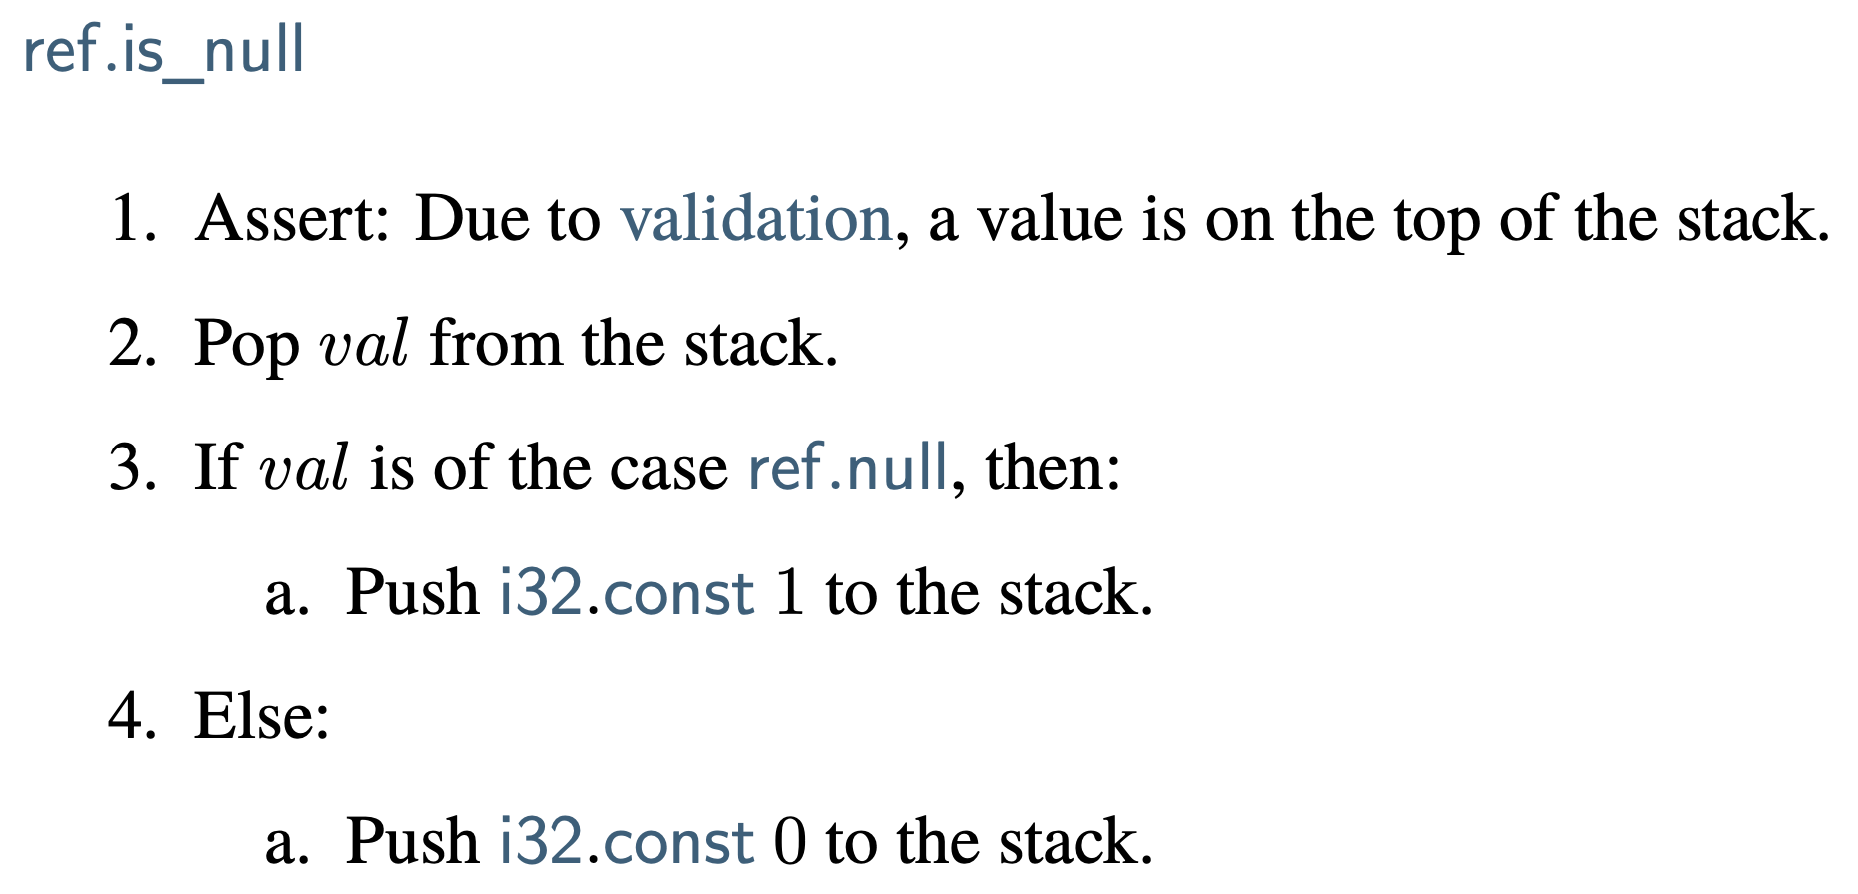
\includegraphics[width=.5\textwidth]{../img/genprose}
\vspace*{-1em}
\caption{Semantics of \inblue{\ensuremath{\mathsf{ref.is\_null}}} in a generated prose specification}
\label{fig:genprose}
\end{figure}

As \al is designed to resemble prose notation, 
generating the English prose specification from \al algorithms is a straightforward task.
Fig.~\ref{fig:genprose} shows the prose pseudocode of \inblue{\ensuremath{\mathsf{ref.is\_null}}} instruction,
generated from the specification in Fig.~\ref{fig:dsl},
which is very close to the original handwritten prose in Fig~\ref{fig:spec1}.
AL algorithms are rendered into prose specification document through three steps.
First, the semantics described in \al is printed into English prose in reStructuredText markup.
For example, the third step of \inblue{\ensuremath{\mathsf{ref.is\_null}}} is printed as follows:
\begin{verbatim}
3. If :math:`val` is of the case \
   :math:`\xref{exec/runtime}{syntax-ref}{\mathsf{ref{.}null}}`, then:
\end{verbatim}
Next, as in the LaTeX backend, prose in reStructuredText are spliced into a skeleton specification document.
Finally, the spliced document is processed by the Sphinx documentation tool~\cite{sphinx},
producing human-frieldnly formats like PDF and HTML.

Note that prose in reStructuredText is not simple plaintext,
but has inline math blocks as denoted by the \texttt{:math:} markup.
Expressions in math blocks are typesetted with LaTeX, thereby
making a clear distinction between specification elements and ordinary English phrases.
Furthermore, the prose backend embeds cross-references into the math blocks 
with \texttt{\textbackslash xref\{doc\}\{section\}\{text\}}.
This serves as a reference to a \texttt{section}
in some reStructuredText file \texttt{doc}, to be rendered as \texttt{text}.
As in the original specification document, 
\inblue{\ensuremath{\mathsf{ref{.}null}}} in the third step references its syntax production rule in a separate file.
This systematic insertion of references rules out
possibilities of missing, broken, or misplaced links when inserted manually.

\subsection{Interpreter Backend}\label{sec:interp} %1p
\dslname supports the interpretation of Wasm programs by \textit{meta-level interpretation}.
By interpreting an \al program that denotes the Wasm semantics, with
a Wasm program as its input value, we can indirectly interpret the Wasm program.

This approach was previously used by the ESMeta framework~\cite{esmeta,jiset}.
ESMeta extracts two main components from the ECMAScript specification~\cite{ecmascript}:
a parser and executable semantics.
The parser is generated from the grammar section in the specification,
which takes a JavaScript program as input and returns a parsed AST as output.
The executable semantics is generated from the structured English prose algorithms in the specification,
and is translated into an internal representation, \ires.
\ires has its own semantics, so it can be executed by an interpreter implementation.
By executing the extracted semantics written in \ires using the parsed AST as input to the semantics,
we can indirectly execute JavaScript programs.

\dslname allows indirect execution of Wasm programs in a similar way.
A parser parses a Wasm program into an AST, which an \al algorithm takes as input.
Unlike ESMeta, \dslname does not generate a Wasm parser,
but uses the parser of the reference interpreter~\cite{wasmparser}.
The executable semantics written in \al is automaitcally extractd as described in Sec.~\ref{sec:dl2al}.
Based on the \al semantics~\cite{il-tr}, we developed an \al interpreter in OCaml.
By executing the extracted semantics written in \al using the parsed AST as input to the semantics,
we can indirectly execute Wasm programs.

As described in Sec.~\ref{sec:aldef}, we can execute an \al program by calling one of its algorithms.
A Wasm program is executed when instantiating a module~\cite[Sec. 4.5.4]{wasmspec} or
invoking a function on a module instance~\cite[Sec. 4.5.5]{wasmspec}.
Thus, the \al interpreter calls the $\mathit{instantiate}$ algorithm to instantiate a module
or the $\mathit{invoke}$ algorithm to invoke one of the functions within the module.
After calling the algorithm, it returns a value or produces a \textit{trap},
which is the result of executing the Wasm program.

%\begin{itemize}
%\item Borrowed implementation from the reference interpreter
%\item Handwritten parts?
%\end{itemize}
%./watsup spec/* --animate --sideconditions --interpreter

\section{Evaluation}
\label{sec:eval}

\begin{itemize}
  \item SIMD, numerics, one helper function is not specified yet
  \item use reference interpreter for numerics (with version)
  \item explanation about the helper function
  \item manually write AL for the helper function
\end{itemize}

\subsection{Correctness}
Wasm official test is written in Wast\textcolor{red}{(reference of Wast)}, scripting language for testing Wasm, which mainly consists of definitions and assertions.
Definitions are Wasm module definition to run, and assertions check the possible result of \textcolor{red}{executing} a Wasm module.
There are 7 kinds of assertions: AssertMalformed, AssertInvalid, AssertUnlinkable, AssertUninstantiable, AssertTrap, AssertReturn, and AssertExhaustion.
Among them, AssertMalformed, AssertInvalid, and AssertUnlinkable are related to static semantics, so we exclude these assertions.
AssertUninstantiable and AssertTrap are assertion that \textcolor{red}{executing} the module traps.
AssertReturn is an assertion that \textcolor{red}{executing} the module returns an expected value.
One interesting assertion is the AssertExhaustion, an assertion that a module falls into call stack overflow.
Because there is no rule about call stack overflow in the Wasm DSL and current Wasm specification, the exact behavior from the specification is running forever.
Therefore, our tool cannot detect call stack overflow, so we exclude AssertExhaustion.
Long story short, we targeted 3 kinds of assertions named AssertUninstantiable, AssertReturn, and AssertTrap in Wasm official test excluding SIMD.

To evaluate the correctness of \textcolor{red}{SpecTec}, we tested the generated AL by executing the Wasm official test using our \textcolor{red}{test driver}.
The AL interpreter and generated AL pass 21,363 AssertReturn, 2354 AssertTrap, and 34 AssertUninstantiable from the official test in \textcolor{red}{???} seconds, which shows the correctness of generated AL.

\subsection{Usefulness}
To assess the effectiveness of SpecTec in preventing human errors, we conducted
an in-depth investigation into actual errors that had previously occurred in
the main branch of the repository for Wasm standard. Our objective was to
determine whether SpecTec could have prevented these errors. We classified the
investigated errors into four distinct categories.

\textbf{Type Errors}
Two fixes were attributed to type errors within the specification. These
instances included an arity mismatch when invoking the auxiliary helper
function runelem, and an omission of the field TYPE during the initialization
of the element instance in the elem.drop execution semantics. We artificially
introduced each of these errors into the DSL spec document and applied SpecTec.
Subsequently, we confirmed that SpecTec effectively identified and reported the
TypeErrors. In addition, the error message gives the information about the
exact location of the error within the specification, and the reason for the
error correctly.  This result signifies its capability to detect mistakes made
by spec writers.

\textbf{Prose Errors}
Five errors were found to occur within the prose notation. These errors
encompassed free identifier issues, the absence of an immediate value after an
instruction name, and outdated steps that introduced a new variable which was
never utilized. Our automatic prose generation process proved to be free from
these types of errors, and we verified that the corresponding prose was
generated accurately, devoid of any such issues.

\textbf{Semantics Errors}
Three errors resulted in incorrect behavior of the WebAssembly specification.
We manually introduced these errors into the DSL, and subsequently executed the
official tests against them using our indirect interpreter. In all cases, the
tests returned failures as expected, indicating that our indirect interpreter
was proficient in detecting these errors.

\textbf{Editorial Fixes}
A total of \inred{ten} editorial fixes were identified. While these fixes did
not impact the behavior of the specification, they addressed typographical
errors in LaTeX or ensured consistency in writing style. Once again, SpecTec
can effectively address these types of issues.  Additionally, the consistency
in writing style within the generated spec is guaranteed by design.

The evaluation results demonstrate that SpecTec is effective at preventing a wide
range of human errors within the WebAssembly specification.  Its capabilities
extend to detecting and addressing type errors, prose errors, semantics errors,
as well as editorial fixes. This is a strong evidence that leveraging SpecTec
can significantly enhance the robustness and reliability of the specification
writing process.

\subsection{Generality}
In this section, we present the generality of SpecTec, by applying it to five
WebAssembl proposals currently at or about to enter phase 4 at the time of
writing. These proposals include Tail Call[?], Extended Constant
Expressions[?], Typed Function References[?], Garbage Collection[?], and
Multiple Memories[?].

The process involved two main steps. First, we manually extended the
specification files for each of these proposals. Next, we used SpecTec to
automatically generate both LaTeX and Prose backends. The necessary
modifications in SpecTec were minimal, primarily involving the addition of new
custom operators for notations specific to some of proposals.

The results of our evaluation are as follows:

\textbf{Successful Description using DSL}: Each of the five proposals was
successfully described using the WebAssembly Domain Specific Language (DSL).
This demonstrates the versatility and adaptability of SpecTec in effectively
capturing the semantics of diverse Wasm features.

\textbf{Transformation into LaTeX}: The descriptions of all proposals were
successfully transformed into LaTeX format. This indicates the capability of
SpecTec to generate formal notation specifications from DSL representations,
contributing to the ease of documentation.

\textbf{Semantic Translation Accuracy in AL and Prose}: Out of the 34
instructions affected by the proposals, all but three instructions had their
semantics correctly translated into Algorithmic Language (AL), and subsequently
into prose. For the three instructions with incorrect translations, we
performed a manual correction. Notably, the required changes were minimal, with
a line diff of only nine.

\textbf{Rigorous Testing and \inred{100\%} Pass Rate}: Following the manual
fixes, we conducted comprehensive testing using the tests of proposals against
the generated prose. The pass rate achieved was an impressive 100\%. This
confirms the accuracy and reliability of the generated prose descriptions,
demonstrating their alignment with the intended behavior specified in DSL.

Overall, the evaluation results indicate that the SpecTec approach is highly
effective and generalizable. It successfully accommodates a range of Wasm
proposals, accurately capturing their semantics in both formal and prose
notations. The minimal manual intervention required further underscores the
efficiency and reliability of SpecTec. These findings affirm the potential of
SpecTec as a transformative tool, not only within the domain of current version
of WebAssembly but also in broader contexts.

Furthermore, in the course of comparing the artifacts generated by SpecTec with
the actual proposals, we identified certain discrepancies. Upon closer
examination, it became evident that these disparities arose from errors within
the official proposals themselves, encompassing both formal and prose
notations. In total, we identified and reported four such errors to the
specification writer, all of which were subsequently rectified. This discovery
underscores the capacity of SpecTec to produce more reliable artifacts in
comparison to the potentially error-prone manual process. It highlights the
potential for SpecTec to not only streamline the specification generation
process but also enhance the overall accuracy and trustworthiness of the
resulting documentation in general.

\subsection{Others}
\begin{itemize}
\item anecdotal evidence
\begin{itemize}
\item no need to write prose
\item code review: readability
\end{itemize}

\item qualitative evaluation?
\begin{itemize}
\item compactness of writing? LoC?
\item arity issues?
\end{itemize}

\item more quantitative evaluation
\begin{itemize}
\item coverage of the prose/LaTeX specification
\end{itemize}
\end{itemize}

%!TEX root = main.tex

\section{Related Work}
\label{sec:related}

\textbf{Programming Language Frameworks}
Researchers have presented numerous frameworks to mechanize the
definitions of programming languages.
Once language definitions are mechanized, frameworks can provide various support
such as LaTeX typesetting and type checking of language definitions,
reference implementation in another language, and 
proof assistant code for theorem provers.
Ott~\cite{ott} allows language designers to specify the semantics in inference rules,
and generates code for Coq, HOL, and Isabelle/HOL.
It has been used for case studies like a large fragment of OCaml.
Spoofax~\cite{spoofax} supports agile development of textual
domain-specific languages with the Eclipse IDE support.
Skeleton~\cite{skeleton} specifies language semantics in big-step semantics
and constructs both concrete abstract interpretation.
PLTRedex~\cite{pltredex} describes language semantics in reduction rules,
and It has specified the semantics of Scheme~\cite{r6rs}.
The K framework~\cite{k} can generate various tools,
including interpreters, model checkers, and verifiers, from a language specification
written in its language K. It has specified the core semantics of real-world programming languages
such as C~\cite{kc}, Java~\cite{kjava}, Python~\cite{kpython}, and JavaScript~\cite{kjs}.
While the aforementioned frameworks aim to support general-purpose languages
with declarative semantics, ESMeta~\cite{esmeta} is designed to
support JavaScript with imperative semantics.
By devising a specific algorithmic language, \ires,
to specify the semantics described in the prose ECMAScript standard,
ESMeta can automatically generate diverse tools~\cite{jiset,jest,jstar,jsaver}.
While existing language frameworks are dedicated to a certain semantics style,
\dslname can handle both declarative and algorithmic styles.

\textbf{Wasm Semantics in Existing Language Frameworks}
The Wasm semantics have been mechanized in PLT-Redex and K.
Two PLT-Redex models specify a large core of Wasm~\cite{wasm-pldi17}:
wasm-redex~\cite{wasm-redex-asumu} and Wasm-Redex~\cite{wasm-redex-adam}.
The Wasm semantics defined by the collection of reduction rules is implemented
by the rewrite system of PLT-Redex.
Both models do not specify the Wasm module semantics, thus complete execution of
Wasm programs is not available.
KWasm~\cite{wasm-k} specifies the Wasm runtime semantics, including the module semantics,
in a single rewrite system in the K framework.
Since it does not model the entire Wasm semantics yet,
it fails for a number of tests in the official Wasm test suite.
While both PLT-Redex and K execute the Wasm semantics using their rewriting engines,
\dslname provides indirect interpretation over an algorithmic representation of the semantics.

\textbf{Wasm Semantics Mechanizations}


%% TODO during the camera ready
%% acknowledgements
% \begin{acks}
% This work was supported by National Research Foundation of
% Korea (NRF) (Grants NRF-2017R1A2B3012020 and 2017M3C4A7068177).

%% bibliography style
\bibliographystyle{ACM-Reference-Format}

%% the bibliography file.
\balance
\bibliography{ref}

\end{document}
\endinput
